\cleartoverso

\thispagestyle{empty}

{\small\setlength{\parskip}{0.8em}\setlength{\parindent}{0em}%
{\centering

Aṭṭhakavagga, zbirka osemverznih sutt

Prevod iz palija.

Izdaja:\\
Amaravati Publications\\
Amaravati Buddhist Monastery\\
Great Gaddesden,\\
Hemel Hempstead,\\
Hertfordshire, HP1 3BZ,\\
Velika Britanija\\
www.amaravati.org

%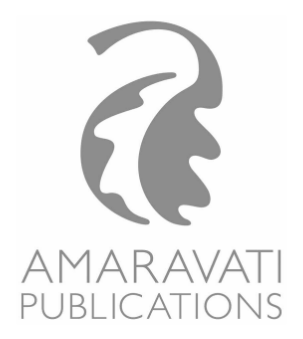
\includegraphics[width=30mm]{abm-pubs-logo.png}

Knjiga je na voljo tudi v elektronski obliki na spletni strani\\
www.slo-theravada.org

ISBN \theISBN

Copyright \copyright\ 2015 Bhikkhu Hiriko

\vfill

Proizvedeno s programom {\fontfamily{cms}\selectfont\LaTeX}. Besedilo je v pisavi Alegreya in Rosarivo, v distribuciji z SIL Open Font Licence.

\theEditionInfo

\thePrintedByInfo

%Para distribuição gratuita\\
%\emph{Sabbadānaṁ dhammadānaṁ jinati}\\
%‘A oferta de Dhamma é superior a qualquer outra oferta.’
%
%Publicado por Amaravati Publications\\
%Amaravati Buddhist Monastery\\
%Hertfordshire, Great Britain\\
%abmpublications@amaravati.org\\
%\href{http://amaravati.org}{www.amaravati.org}
%
%Este livro encontra-se disponível para distribuição gratuita em\\
%\href{http://forestsanghapublications.org/}{www.forestsanghapublications.org}
%
%ISBN \theISBN
%
%Copyright \copyright\ 2014 Amaravati Buddhist Monastery
%
%Imagem de capa de autoria de Anandajoti Bhikkhu\\
%Para mais informações visite \href{http://www.photodharma.net/}{www.photodharma.net}
%
%\vfill
%
%{%\footnotesize
%
%Este trabalho encontra-se licenciado sob a
%Atribuição NãoComercial\\ SemDerivações 2.0 Reino Unido: Inglaterra e País de Gales\\
%\href{http://creativecommons.org/licenses/by-nc-nd/2.0/uk/deed.pt}{www.creativecommons.org/licenses/by-nc-nd/2.0/uk/deed.pt}
%
%Veja página \pageref{copyright-details} para mais detalhes sobre direitos e restrições desta licença.
%
%Produzido com o sistema tipográfico \LaTeX. Fonte utilizada: Gentium, distribuída por SIL International e Crimson Text, criada por Sebastian~Kosch.
%
%%Produced with the \LaTeX\ typesetting system. Typeset in Gentium, distributed by SIL International, and Crimson Text, by Sebastian Kosch.
%
%\theEditionInfo
%
%}

}}


